% Herramientas Computacionales
% Universidad de los Andes
% 2015-1
% Taller 3

\documentclass[14pt]{article}
\usepackage[utf8]{inputenc}
\usepackage{graphicx}
\begin{document}
 
En la fig.\ref{fig:isaac} se muestra el retrato de \textit{Sir Isaac Newton}
 
\begin{figure}[h]
\centering
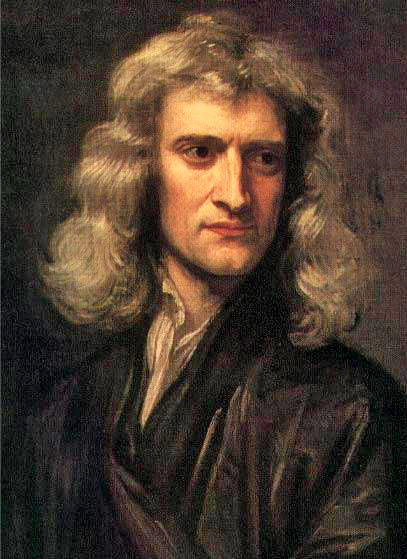
\includegraphics[scale=0.3]{isaac.png}
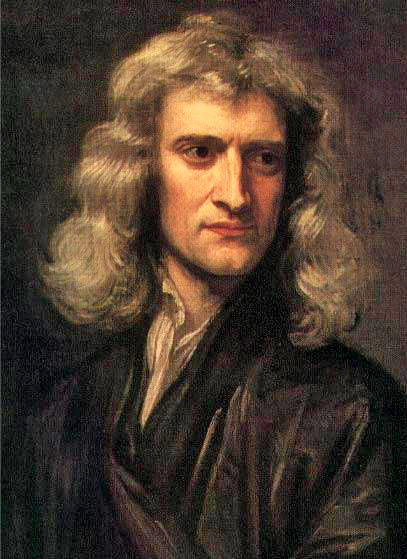
\includegraphics[scale=0.2]{isaac.png}
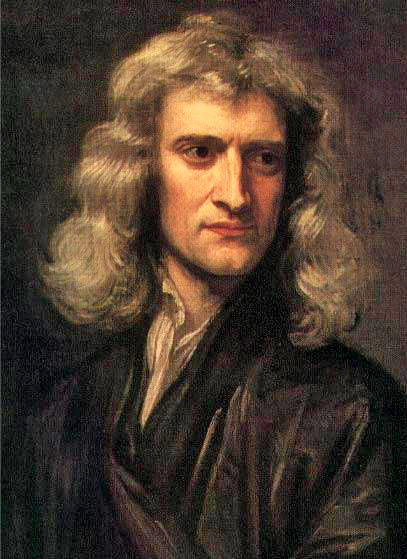
\includegraphics[scale=0.2,angle=100]{isaac.png}
\caption{Retrato de \textit{Sir Isaac Newton}}
\label{fig:isaac}
\end{figure}
 
\end{document}
